
\begin{figure}[p]

    \noindent\makebox[\textwidth]{
        \centering
        %\includegraphics[width=0.8\textwidth]{../../sympy/catalan/coloured.pdf}

        % using *angle* property to rotate it is difficult to properly align it
        % in order to have a "real" matrix representation.
        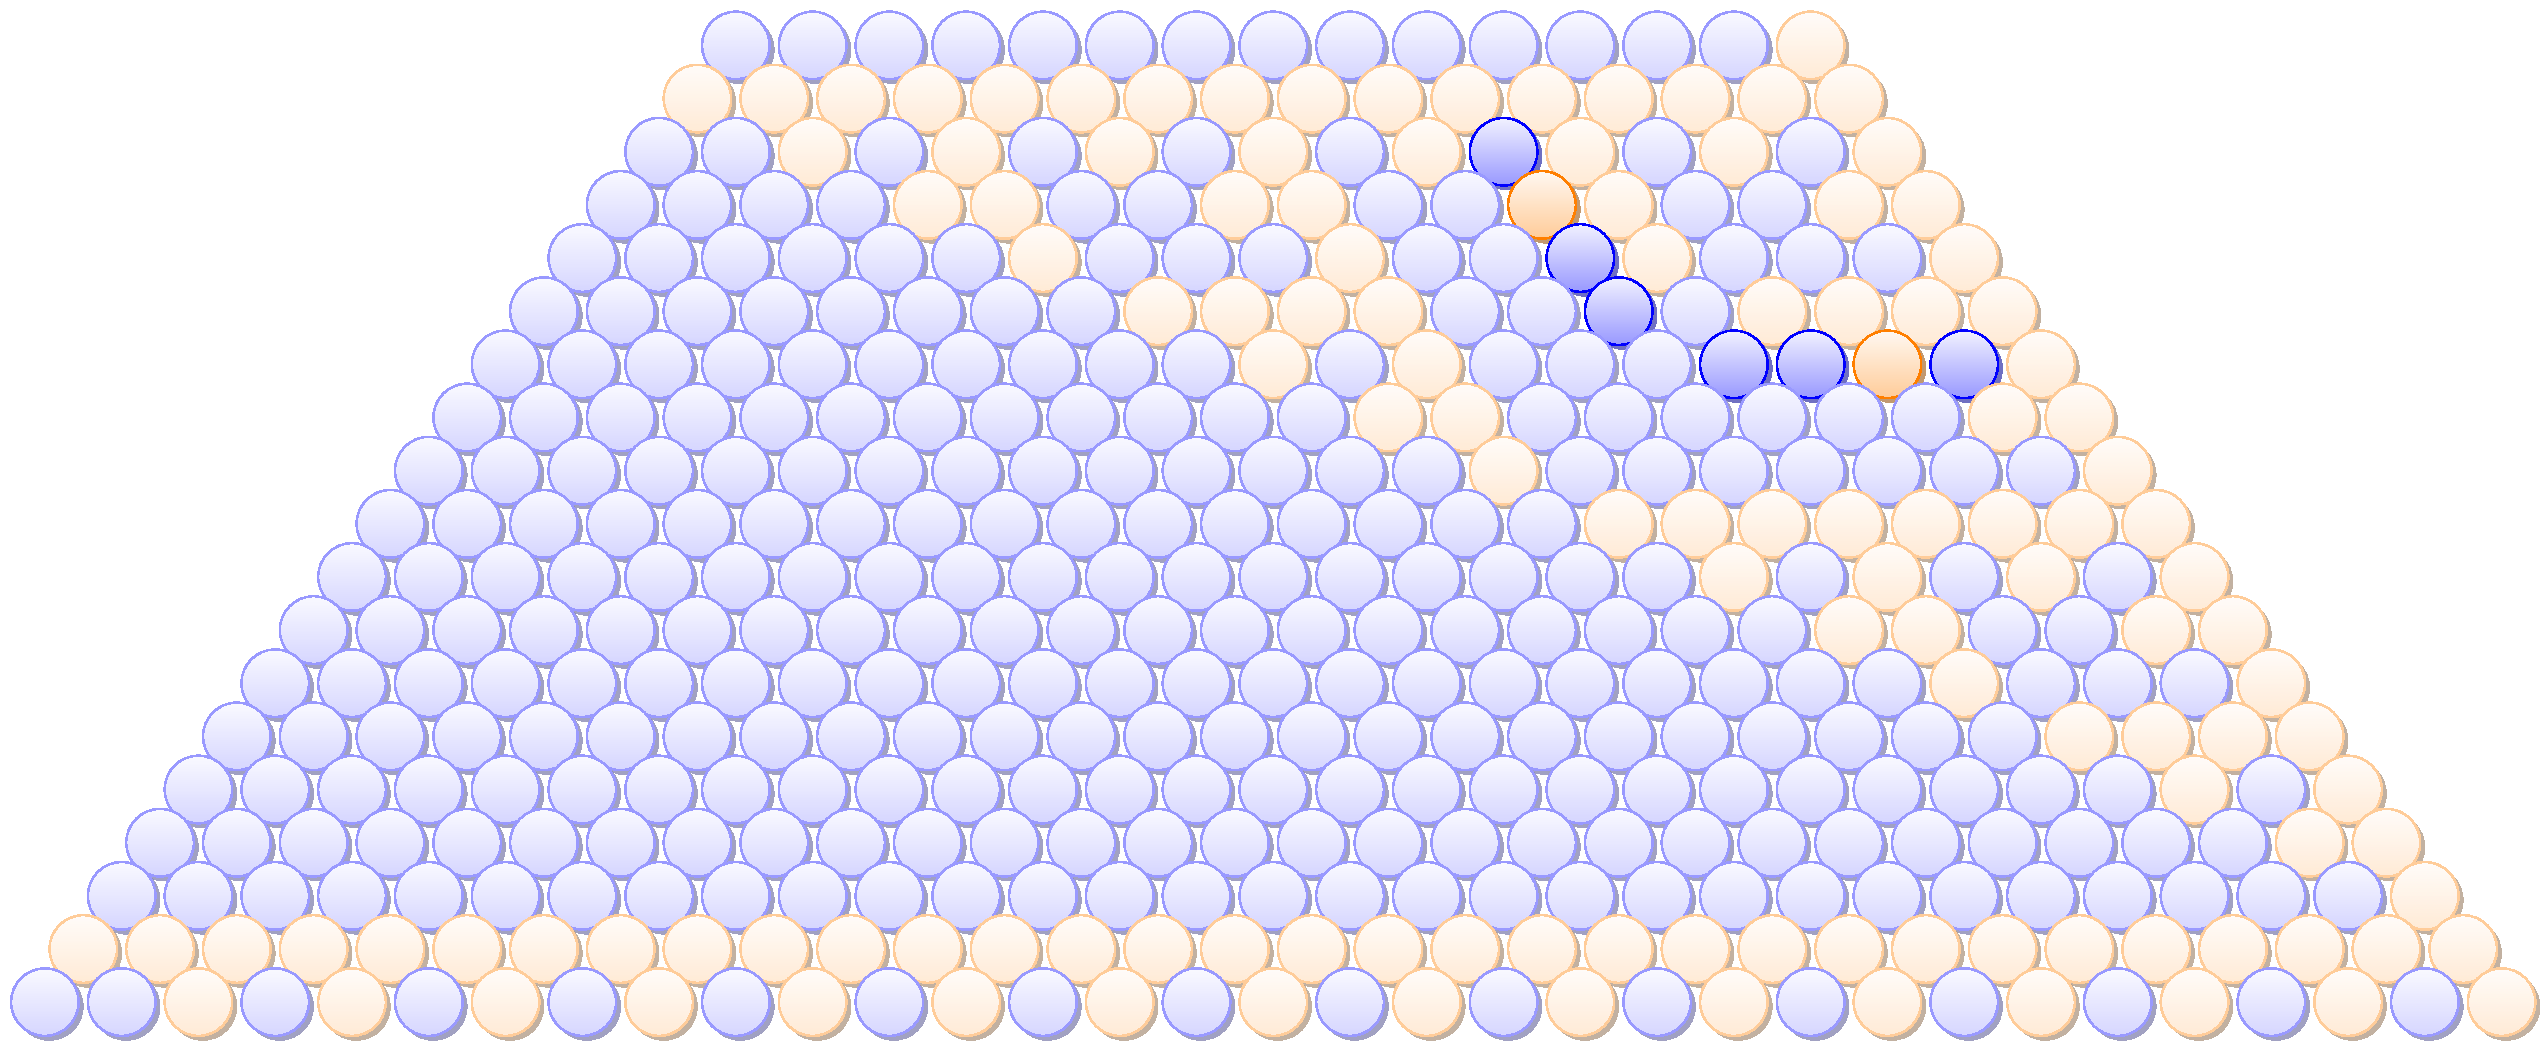
\includegraphics[width=10cm, height=10cm, keepaspectratio=true]
            {../RART2015/catalan-tikz/mirrored-clusters/mirrored-clusters.pdf}
    }

    % this 'particular' line is necessary to use `displaymath' environment
    % into the caption environment, togheter with the inclusion of 
    % `caption' package. See here for more explanation:
    % http://stackoverflow.com/questions/2716227/adding-an-equation-or-formula-to-a-figure-caption-in-latex
    \captionsetup{singlelinecheck=off}
    \caption[\emph{Mirrored} principal clusters $\mathcal{C}_{\equiv_{2}}^{(4)}$]
        {Some coefficients in \emph{mirrored} cluster $\mathcal{C}_{\equiv_{2}}^{(4)}$ 
        over $\hat{d}_{20,2^{4}-1}$: congruences $d_{20-e,2^{4}-1-e} \equiv_{2} d_{20,2^{4}-1+e}$ 
        for $e\in\lbrace1,\ldots,4\rbrace$ }

    \label{fig:catalan-mirrored-clusters}

\end{figure}
